\documentclass{article}
\usepackage{graphicx} % Required for inserting images
\usepackage{amsmath}
\usepackage{amsthm}
\usepackage{amsfonts}
\usepackage{amssymb}
\usepackage{hyperref}
\usepackage{float}
\usepackage{tikz}
\usepackage{pgfplots}
\usetikzlibrary{calc, arrows.meta, decorations.markings, 3d}
\pgfplotsset{compat=1.18}

\title{Multivariable Calculus Prerequisites for Studying Brownian Motion on Manifolds}
\author{Jean-Jacques St Leroux}
\date{May 2026}

\begin{document}

\maketitle

\section{Introduction}

This document is the multivariable calculus companion to the linear algebra prerequisites document. We assume fluency in single-variable calculus (limits, derivatives, integrals, Taylor series). The point of this document is to refresh the multivariable calculus one needs to study Brownian motion on manifolds as we do in our project.

The topics covered are as follows. In Section 2, we review partial derivatives, the gradient, and the linearization of a function at a point. In Section 3, we discuss the Jacobian matrix and the multivariable chain rule. In Section 4, we cover parametric curves in $\mathbb{R}^n$: velocity, arc length, and curvature. In Section 5, we cover parametrized surfaces, regularity, the tangent plane, and the unit normal vector. In Section 6, we cover multiple integrals and the change-of-variables formula. In Section 7, we discuss the surface area element and surface integrals. In Section 8, we cover the vector calculus operators (divergence, curl, and the Laplacian), which is what we generalize later to define Brownian motion's generator on a manifold.

Throughout, the convention is that vectors are typeset in bold ($\mathbf{x}, \mathbf{v}, \mathbf{r}$) and scalars are not. Where useful, we will write a function $f: \mathbb{R}^n \to \mathbb{R}^m$ to be explicit about the domain and codomain.

\section{Partial Derivatives, the Gradient, and Linearization}

Single-variable calculus has one notion of derivative because there is one direction to move in. In multivariable calculus, a function can be differentiated along any direction in its domain, so the question ``what is the rate of change of $f$?'' has many answers. The first step is to fix coordinate directions.

\subsection{Partial Derivatives}

Let $f: \mathbb{R}^n \to \mathbb{R}$ be a function of $n$ variables, written $f(x_1, \ldots, x_n)$. The \textit{partial derivative} of $f$ with respect to $x_i$ at the point $\mathbf{a} = (a_1, \ldots, a_n)$ is
$$\frac{\partial f}{\partial x_i}(\mathbf{a}) = \lim_{h \to 0} \frac{f(a_1, \ldots, a_i + h, \ldots, a_n) - f(\mathbf{a})}{h}.$$
This is simply the single-variable derivative of $f$ with respect to $x_i$ where all other variables are treated as constants. Geometrically, fixing all but one variable cuts the graph of $f$ with a plane parallel to the $x_i$-axis; the partial derivative is the slope of the resulting curve in that slice.

One often writes $\partial_i f$ or $f_{x_i}$ as shorthand, and the same shorthand extends to higher-order partial derivatives: $\partial_{ij}^2 f = \partial^2 f / \partial x_i \partial x_j$, and so on. For sufficiently smooth $f$ (which all of our functions will be), the mixed partials commute, i.e. $\partial_{ij}^2 f = \partial_{ji}^2 f$. This is Clairaut's theorem and we shall use it without comment from here on.

\subsection{The Gradient Vector}

Should one compile all $n$ partial derivatives into a single vector, we obtain the \textit{gradient} of $f$ at $\mathbf{a}$, written $\nabla f(\mathbf{a})$:
$$\nabla f(\mathbf{a}) = \left( \frac{\partial f}{\partial x_1}(\mathbf{a}),\; \frac{\partial f}{\partial x_2}(\mathbf{a}),\; \ldots,\; \frac{\partial f}{\partial x_n}(\mathbf{a}) \right) \in \mathbb{R}^n.$$
The gradient is the fundamental first-derivative object for a scalar-valued function of several variables, and it has two properties that we will use constantly.

First, $\nabla f(\mathbf{a})$ \textit{points in the direction of steepest ascent} of $f$ at $\mathbf{a}$, and its magnitude $|\nabla f(\mathbf{a})|$ is the rate of increase in that direction. Second, $\nabla f(\mathbf{a})$ is \textit{perpendicular to the level set} $\{\mathbf{x} : f(\mathbf{x}) = f(\mathbf{a})\}$ at $\mathbf{a}$. Both properties are explained using the directional derivative formula in the next subsection.

\begin{figure}[H]
\centering
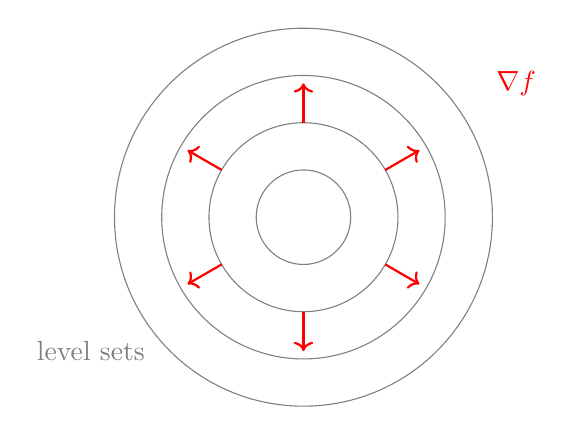
\begin{tikzpicture}[scale=1.0]
    % Level curves (concentric circles)
    \foreach \r in {0.6, 1.2, 1.8, 2.4} {
        \draw[gray, thin] (0,0) circle (\r);
    }
    % Gradient arrows at a few points
    \foreach \angle in {30, 90, 150, 210, 270, 330} {
        \draw[->, red, thick] ({1.2*cos(\angle)}, {1.2*sin(\angle)})
            -- ({1.7*cos(\angle)}, {1.7*sin(\angle)});
    }
    \node[red] at (2.7, 1.7) {$\nabla f$};
    \node[gray] at (-2.7, -1.7) {level sets};
\end{tikzpicture}
\caption{For $f(x,y) = x^2 + y^2$, the level sets are concentric circles and the gradient (red) points radially outward, perpendicular to the level sets, in the direction of steepest ascent.}
\label{fig:gradient}
\end{figure}

\subsection{Directional Derivatives}

The directional derivative measures the instantaneous rate at which a function changes along a specified vector through a given point. If the vector is multiplied by a scalar, the corresponding directional derivative is multiplied by the same scalar.

Given a scalar function $f(x)=f(x_1, x_2, \dots, x_n)$ and a vector \textbf{v}, the directional derivative is the function $D_\mathbf{v} f(\mathbf{a}) = \nabla f(\mathbf{a}) \cdot \mathbf{v}$, which is defined by the limit 
$$D_\mathbf{v} f(\mathbf{a})=\lim_{h \to 0}  \frac{f(x+h\textbf{v})-f(x)}{h}= \left. \frac{d}{dt}f(x+t\textbf{v})\right|_{t}
$$
If the function f is differentiable at x, then the directional derivative exists along any vector v at x, and this is where we obtain the formulation.

Three important pieces of information follow. First, This formula recovers the partial derivative $\partial f / \partial x_i$ when $\mathbf{v} = \mathbf{e}_i$ ($\mathbf{e}_i$ being the standard basis vector). Let us explain. The standard basis vector has a 1 in the
i-th slot and zeros elsewhere, hence 
$$\nabla f(\mathbf{a}) \cdot \mathbf{e}_i=\sum_{j=1}^{n} \frac{\partial f}{\partial x_j}(\mathbf{e}_i)(\textbf{a}) =\frac{\partial f}{\partial x_i}$$
since only the i-th component survives after applying this operation. 

Second, the gradient points in the direction of steepest descent. By the angle formula for the dot product, $D_\mathbf{u} f(\mathbf{a})=\nabla f(\mathbf{a}) \cdot \mathbf{u}=|\nabla f(\mathbf{a})|\cos(\theta)$, where $\theta$ is the angle between the vectors $\nabla f(\mathbf{a})$ and \textbf{u}. This quantity is maximized when $\cos(\theta)=1$, or at $\theta=0$, i.e. when the vector \textbf{u} points in the gradient's direction. So the gradient direction is hence the direction of steepest ascent, and the gradient's magnitude is the rate of increase in that direction. The bound on how great this magnitude can be is given by Cauchy-Schwarz, where $|\nabla f \cdot\textbf{u}| \leq |\nabla f||\textbf{u}|$.

Third, the gradient is perpendicular to level sets. Given a non-trivial gradient, let $\gamma=(-\epsilon, \epsilon) \to \mathbb{R}^n$ be any smooth curve lying in the level set $\{f=c\}$, where $\gamma$ is a small open interval around 0 such that $\gamma(0)=\textbf{a}$, and $\epsilon$ is some unspecified small positive number. It follows $f(\gamma(t))=c$ for all values of $t$. At $t=0$, we can differentiate both sides using the chain rule (as we shall elaborate more on in the next section) which gives 
$$\frac{d}{dt}f(\gamma(t))=\nabla f(\gamma(t)) \cdot \gamma '(t).$$
At $t=0$, we have $0=\nabla f(\textbf{a}) \cdot \gamma '(0)$. We thus see the dot product of the gradient vector and the tangent vector $\gamma'(t)$ on the level curve is zero. Since this works for any walk $\gamma$ along the level set through $\mathbf{a}$, it works for every tangent direction at $\mathbf{a}$. So the gradient is perpendicular to the level set at $\mathbf{a}$.

\subsection{Linearization and the Tangent Plane}

For $f: \mathbb{R}^n \to \mathbb{R}$ differentiable at $\mathbf{a}$, the best linear approximation near $\mathbf{a}$ is
$$f(\mathbf{x}) \approx f(\mathbf{a}) + \nabla f(\mathbf{a}) \cdot (\mathbf{x} - \mathbf{a}).$$
Let's see where this definition comes from, focusing on the case when $n = 2$. In such case, we have a vector $\textbf{a}=(a_1, a_2)$ -- where the approximation is taken at -- and a vector $\textbf{x}=(x,y)$, which is the displacement vector from \textbf{x} to the input. The gradient is $\nabla f(\textbf{a})=(\partial_x f(a), \partial_y f(a))$, and the displacement vector is $\textbf{x}-\textbf{a}=(x-a_1, y-a_2)$. If we take the dot product between the gradient vector and the displacement vector, we obtain 
$$\nabla f(\textbf{a}) \cdot (\textbf{x}-\textbf{a})=\frac{\partial f}{\partial x}(\textbf{a})(x-a_1) + \frac{\partial f}{\partial y} (\textbf{a})(y-a_2).$$
So the linear approximation at $z=f(x,y)$ is given by the sum of $f(a_1, a_2)$ and the dot product; namely
$$z=f(x,y) \approx f(a_1,a_2)+\frac{\partial f}{\partial x}(\textbf{a})(x-a_1) + \frac{\partial f}{\partial y}(\textbf{a})(y-a_2).$$
This is the equation of the tangent plane to the graph $z = f(x, y)$ at the point $(\mathbf{a}, f(\mathbf{a}))$. 

It is worthwhile to connect this construction of a linear approximation to that of the derivative's using limits. Recall that $f : \mathbb{R}^n \to \mathbb{R}^n$ is differentiable at $\textbf{a}$ if 
$$\lim_{\textbf{x} \to \textbf{a}}\frac{|f(\textbf{x)}-f(\textbf{a})|}{|\textbf{x}-\textbf{a}|}=\nabla f(\textbf{a})$$
or equivalently,
$$\lim_{\textbf{x} \to \textbf{a}}\frac{|f(\textbf{x)}-f(\textbf{a})-\nabla f(\textbf{a}) \cdot (\textbf{x}-\textbf{a})|}{|\textbf{x}-\textbf{a}|}=0$$
The numerator is the error of the linear approximation at \textbf{x}. It is precisely f(\textbf{x}) minus the tangent plane's approximation at \textbf{x} as we have seen just above. The denominator is the distance from \textbf{x} to \textbf{a}, and the limit says this ratio tends to zero. In other words, we are saying the error of the linear approximation shrinks faster than the distance between the points does. This entitles us to call such a linear approximation the "best linear approximation", where "best" comes from the following uniqueness fact: the linearization is the*only affine function whose error decays faster than $|\mathbf{x} - \mathbf{a}|$. Any other plane through $(\mathbf{a}, f(\mathbf{a}))$ has error at least proportional to $|\mathbf{x} - \mathbf{a}|$, so its ratio in the limit stays bounded away from zero. This allows us to call $\nabla f(\mathbf{a})$ the total derivative of $f$ at $\mathbf{a}$: it is the unique vector that makes the linear approximation "good" in this sense.

\begin{figure}[H]
\centering
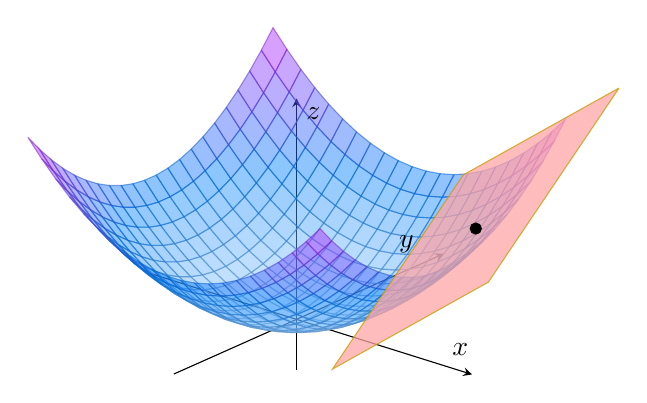
\begin{tikzpicture}
\begin{axis}[
    view={40}{30},
    width=0.75\textwidth,
    axis lines=middle,
    domain=-1.5:1.5, y domain=-1.5:1.5,
    samples=22, samples y=22,
    ticks=none,
    xlabel={$x$}, ylabel={$y$}, zlabel={$z$},
    z buffer=sort,
    enlargelimits=false,
]
% Surface z = x^2 + y^2
\addplot3[surf, opacity=0.55, fill opacity=0.45,
          colormap/cool, shader=faceted] {x^2 + y^2};
% Tangent plane at (a_1, a_2) = (1, 1): z = 2x + 2y - 2
\addplot3[surf, opacity=0.75, fill=red!35, draw=red!70,
          samples=2, samples y=2,
          domain=0.2:1.8, y domain=0.2:1.8] {2*x + 2*y - 2};
% Point of tangency
\addplot3[only marks, mark=*, mark size=2pt, black]
    coordinates {(1, 1, 2)};
\end{axis}
\end{tikzpicture}
\caption{The graph $z = x^2 + y^2$ (blue) and its tangent plane (red) at the point $(\mathbf{a}, f(\mathbf{a}))$. The plane touches the graph at exactly that point and matches its partial slopes there.}
\label{fig:tangent-plane-3d}
\end{figure}

\section{The Total Derivative, the Jacobian, and the Chain Rule}

In our project, we write the same stochastic process in different coordinate systems (spherical coordinates on $S^2$, $(u, v)$ coordinates on $T^2$), and therefore we must to know how the stochastic differential equation transforms under a coordinate change. The Stratonovich chain rule transforms cleanly, while the Itô chain rule does not, and the discrepancy is what justifies our choice of stochastic calculus. So a precise grasp of the multivariable chain rule is essential.

\subsection{The Jacobian Matrix}

Let $f: \mathbb{R}^n \to \mathbb{R}^m$ be a function. We can write $f$ in components as $f(\mathbf{x}) = (f_1(\mathbf{x}), \ldots, f_m(\mathbf{x}))$, where each $f_i: \mathbb{R}^n \to \mathbb{R}$ is a scalar-valued function. The \textit{Jacobian matrix} of $f$ at $\mathbf{a}$, denoted as $\mathbf{J}_f(\mathbf{a})$, is the $m \times n$ matrix of all first-order partial derivatives:
$$\mathbf{J}_f(\mathbf{a}) = \begin{pmatrix}
\dfrac{\partial f_1}{\partial x_1}(\mathbf{a}) & \cdots & \dfrac{\partial f_1}{\partial x_n}(\mathbf{a}) \\[1em]
\vdots & \ddots & \vdots \\[0.5em]
\dfrac{\partial f_m}{\partial x_1}(\mathbf{a}) & \cdots & \dfrac{\partial f_m}{\partial x_n}(\mathbf{a})
\end{pmatrix}.$$
The $i$-th row of the Jacobian is the gradient of the $i$-th component function $f_i$. When $m = 1$, the Jacobian is a single row, namely $(\nabla f)^\top$. When $m = n$, the Jacobian is square, and its determinant ($\det \textbf{J}_f$) is what shows up in the change-of-variables formula in Section 6.

The Jacobian deserves to be categorized alongside the term ``derivative'' because of the following fact, which is the proper multivariable definition of differentiability. We may furthermore say $f$ is differentiable at $a$ if there is a linear map $L : \mathbb{R}^n \to \mathbb{R}^m$ such that
$$\lim_{\mathbf{h} \to \mathbf{0}} \frac{|f(\mathbf{a} + \mathbf{h}) - f(\mathbf{a}) - L(\mathbf{h})|}{|\mathbf{h}|} = 0,$$
in which case $L$ is the linear map represented by the matrix $\mathbf{J}_f(\mathbf{a})$. Differentiability in this sense is stronger than the mere existence of partial derivatives, for the two are not equivalent. A sufficient condition for it to hold is that the partials exist and are continuous in a neighborhood of $\mathbf{a}$ (in which case $f$ is called continuously differentiable, or $C^1$).

\subsection{The Multivariable Chain Rule}

If $g: \mathbb{R}^n \to \mathbb{R}^m$ and $\mathbf{f}: \mathbb{R}^m \to \mathbb{R}^k$ are both differentiable, then the composition $h = f \circ g : \mathbb{R}^n \to \mathbb{R}^k$ is differentiable, and its Jacobian satisfies
$$\textbf{J}_f(\mathbf{a}) = \textbf{J}_f(g(\mathbf{a})) \cdot \textbf{J}_g(\mathbf{a}).$$
That is, the chain rule says that the derivative of a composition is the matrix product of the individual derivatives, evaluated at the appropriate points. Quickly, note that the matrix sizes are compatible: $\textbf{J}_f$ is $k \times m$, $\textbf{J}_g$ is $m \times n$, and their product is $k \times n$, which matches $\textbf{J}_h$.

Using components in the notation, with $\mathbf{y} = \mathbf{g}(\mathbf{x})$ and $\mathbf{z} = \mathbf{f}(\mathbf{y})$, the chain rule reads
$$\frac{\partial z_i}{\partial x_j} = \sum_{\ell = 1}^m \frac{\partial z_i}{\partial y_\ell} \cdot \frac{\partial y_\ell}{\partial x_j}.$$
This is the form you have likely seen in a multivariable calculus course. Compared to the matrix form, they are equivalent expressions but the matrix form makes it obvious the chain rule is matrix multiplication. Whenever you encounter the chain rule in a stochastic-analysis context, the thought being posed is the same: how does a derivative transform under composition?

\subsection{Why This Matters for the Project}

Suppose a particle moves in $\mathbb{R}^n$ according to some random process $\mathbf{X}_t$, and we want to study a smooth function $f(\mathbf{X}_t)$. In ordinary calculus, the chain rule says
$$\frac{d}{dt} f(\mathbf{X}_t) = \nabla f(\mathbf{X}_t) \cdot \frac{d\mathbf{X}_t}{dt}.$$
For Brownian motion, however, $\mathbf{X}_t$ is nowhere differentiable, so this formula cannot work. Instead, we may choose between two competing replacements: \textit{Itô's formula}, which adds a second-derivative correction term involving the Hessian of $f$, and \textit{Stratonovich's formula}, which looks identical to the classical chain rule. The Stratonovich formula is able to transform under coordinate changes because it obeys the chain rule in the same form as the classical multivariable chain rule. This is why our simulation on the sphere and torus is naturally written in Stratonovich form.

\section{Parametric Curves in $\mathbb{R}^n$}

A parametric curve in $\mathbb{R}^n$ is a continuous function $\gamma: I \to \mathbb{R}^n$, where $I \subseteq \mathbb{R}$ is an interval. The image $\gamma(I)$ is the geometric curve, and $\gamma$ itself is the curve's \textit{parametrization}. Curves are the simplest case of multivariable objects whose intrinsic geometry (length, curvature) differs from how they are represented in coordinates. We shall explore these properties in depth throughout this section

\subsection{Velocity, Speed, and Acceleration}

The velocity of $\gamma$ at $t$ is $\gamma'(t) \in \mathbb{R}^n$, the speed is $|\gamma'(t)|$, and the acceleration is $\gamma''(t)$. Let us verify  these reduce to the usual single-variable quantities when $n = 1$, and then we will compute them for the helix $\gamma(t) = (\cos t, \sin t, t)$.

First, write $\gamma(t) = (\gamma_1(t), \ldots, \gamma_n(t))$ in components. Then everything is componentwise:
$$\gamma'(t) = (\gamma_1'(t), \ldots, \gamma_n'(t)), \qquad \gamma''(t) = (\gamma_1''(t), \ldots, \gamma_n''(t)).$$
The velocity $\gamma'(t)$ is a vector pointing in the direction of motion with length equal to the motion's speed. The speed is therefore the magnitude, computed by the familiar expression $|\gamma'(t)| = \sqrt{\gamma_1'(t)^2 + \cdots + \gamma_n'(t)^2}$. Since speed is the magnitude of the velocity vector, it is a scalar. We can then think of the acceleration, $\gamma''(t)$, intuitively; it encodes both the speeding up or slowing down and turning of the velocity vector. The reason being is because velocity may be decomposed into length and direction, where $\gamma '(t)=|\gamma'(t)| \cdot \frac{\gamma'(t)}{|\gamma'(t)|}$. The first term is the velocity (denote this $v(t)$, the second is the unit tangent (denote this $\textbf{T}(v)$). Taking the derivative requires us to use the product rule, hence $\gamma''(t)=v'(t)\textbf{T}(t)+v(t)\textbf{T}'(t)$. The first term is parallel to velocity; it captures a change of speed. The second term is perpendicular to velocity, for $\mathbf{T}$ is a unit vector, hence $|\mathbf{T}|^2 = 1$ is constant, so differentiating both sides gives $\mathbf{T} \cdot \mathbf{T}' = 0$. This term captures change in direction. It points in the direction the velocity is rotating. 

When $n = 1$, $\gamma(t) = \gamma_1(t)$ is just a real-valued function. Then $\gamma'(t) = \gamma_1'(t)$ is the ordinary derivative, the speed is $|\gamma'(t)|$ (a straightforward absolute value, for there are no components to combine), and the acceleration is $\gamma''(t)$. 

Consider this for the helix $\gamma(t) = (\cos t, \sin t, t)$:
\begin{align*}
    \gamma'(t) &= (-\sin t,\, \cos t,\, 1) \\
    |\gamma'(t)| &= \sqrt{\sin^2 t + \cos^2 t + 1} = \sqrt{2} \\
    \gamma''(t) &= (-\cos t,\, -\sin t,\, 0)
\end{align*}
Two observations are worth a mention. The speed $\sqrt{2}$ is constant, so the helix is traversed at uniform pace. The acceleration is horizontal (its $z$-component is zero), points inward toward the $z$-axis at every $t$, and has constant magnitude $|\gamma''(t)| = 1$. At constant speed, the velocity cannot lengthen or shorten, so all the acceleration does is turn it.

\subsection{Arc Length and the Arc-Length Parametrization}

The arc length of $\gamma$ from $t = a$ to $t = b$ is
$$L = \int_a^b |\gamma'(t)|\, dt.$$
The integrand $|\gamma'(t)|\, dt$ is the infinitesimal distance traveled in time $dt$ (speed times time), and the integral sums these contributions.

As an example, consider the circle of radius $R$ parametrized as $\gamma(t) = (R \cos t, R \sin t)$ on $[0,2\pi]$:
$$\gamma'(t) = (-R \sin t,\, R \cos t), \quad |\gamma'(t)| = R, \quad L = \int_0^{2\pi} R\, dt = 2\pi R,$$
recovering the familiar circumference. For the helix, $|\gamma'(t)| = \sqrt{2}$ from above, so $L\big|_0^T = \sqrt{2}\, T$, where $T$ represents the interval traversed. One full turn ($T = 2\pi$) covers $2\pi\sqrt{2}$, longer than the unit circle's circumference because of the vertical climb.

\textit{Reparametrization by arc length.} Say that we have the goal to replace the parameter $t$ with arc length $s$ so the resulting curve has speed $1$ everywhere. Why does this happen? Let us think about this intuitively. Speed measures distance traveled per unit of some parameter, usually time. In an arbitrary parametrization, the parameter $t$ and the distance traveled $s$ are different things (say, clock time vs. cumulative distance) so $ds/dt$ depends on how fast you are moving. However, should you make $s$ itself the parameter, then the parameter and the distance are equivalent variables. Distance traveled per unit of time becomes distance traveled per unit of distance, which is standardizes the curve to make speed irrelevant. Each unit you advance the parameter by, you have moved exactly one unit along the curve, because the parameter is the distance along the curve.

Think of arc length parameterization with a driving analogy. Your car has both a clock and an odometer. Position along a route as a function of clock time has speed measured in miles per hour, which varies as you accelerate and brake. Position-along-route as a function of odometer reading has speed measured in miles per mile, which is identical to 1, because each new mile on the odometer is by definition exactly one mile farther down the road. It is the same trip with two parametrizations and differing notions of "speed", but only the odometer-parametrization gives a constant.

Define
$$s(t) = \int_0^t |\gamma'(u)|\, du$$
as the arc length traveled from time $0$ to time $t$. Assuming $\gamma'(u) \neq 0$ throughout, $s(t)$ is strictly increasing, hence it has an inverse. Solve for $t$ in terms of $s$ to get $t(s)$, and define $\tilde{\gamma}(s) = \gamma(t(s))$.

To check that $\tilde{\gamma}$ has unit speed, apply the chain rule:
$$\tilde{\gamma}'(s) = \gamma'(t(s)) \cdot t'(s).$$
By the fundamental theorem of calculus, $s'(t) = |\gamma'(t)|$, so $t'(s) = 1 / |\gamma'(t(s))|$. Therefore
$$|\tilde{\gamma}'(s)| = |\gamma'(t(s))| \cdot \frac{1}{|\gamma'(t(s))|} = 1.$$
So $\tilde{\gamma}$ traces the same set of points as $\gamma$, but at constant unit speed, and the parameter $s$ measures arc length.

Consider again the circle of radius $R$: $s(t) = R t$, so $t(s) = s/R$, and
$$\tilde{\gamma}(s) = (R \cos(s/R),\, R \sin(s/R)),$$
which has unit speed (verify by direct computation, noticing the chain rule cancels terms).

As for the helix $s(t) = \sqrt{2}\, t$, we have $t(s) = s/\sqrt{2}$, and
$$\tilde{\gamma}(s) = (\cos(s/\sqrt{2}),\, \sin(s/\sqrt{2}),\, s/\sqrt{2}).$$
Verify $|\tilde{\gamma}'(s)| = 1$ as a check.

In summary, the arc-length parametrization strips away how fast you traversed the curve and leaves only the curve's intrinsic geometry. Two different parametrizations of the same geometric curve can have vastly different speeds, but the arc-length parametrization is canonical (up to choice of starting point and direction of travel). That enables the next subsection, for definitions like curvature only make sense once arbitrary speed choices have been accounted for.

\subsection{Curvature and the Frenet Frame}

For a unit-speed curve $\gamma(s)$ in $\mathbb{R}^3$, define the unit tangent
$$\mathbf{T}(s) = \gamma'(s).$$
$\mathbf{T}$ is a unit vector by assumption, since $|\gamma'(s)| = 1$.

The fact that $|\mathbf{T}|^2 = \mathbf{T} \cdot \mathbf{T} = 1$ is constant has an immediate consequence. Differentiating both sides with respect to $s$,
$$0 = \frac{d}{ds}(\mathbf{T}^2) = 2\, \mathbf{T} \cdot \mathbf{T}',$$
which gives $\mathbf{T}'(s) \perp \mathbf{T}(s)$. The rate of change of the unit tangent is always perpendicular to the tangent itself. Geometrically, this is the statement that a unit vector can only change by rotating, never by stretching, and the direction of rotation is perpendicular to it. Hence the magnitude of $\mathbf{T}'(s)$ measures how quickly the tangent is rotating, which is curvature:
$$\kappa(s) = |\mathbf{T}'(s)| = |\gamma''(s)|.$$
A straight line has $\kappa = 0$ (the tangent does not rotate at all); a sharp turn corresponds to large $\kappa$.

When $\kappa \neq 0$, normalize $\mathbf{T}'(s)$ to get the unit normal:
$$\mathbf{N}(s) = \frac{\mathbf{T}'(s)}{\kappa(s)}.$$
$\mathbf{N}$ is a unit vector perpendicular to $\mathbf{T}$, pointing in the direction the curve is bending. The plane spanned by $\mathbf{T}$ and $\mathbf{N}$ is the \textit{osculating plane}.

Instantaneously, the curve looks like a circle of radius $1/\kappa$ lying in that plane. For a circle of radius $R$ parametrized at unit speed, direct computation gives curvature $\kappa = 1/R$, so curvature and radius are reciprocals. The \textit{osculating circle} to a curve at a point is the unique circle that matches the curve in position, tangent direction, and curvature there. It is the best second-order approximation to the curve, the natural next step after the tangent line (which matches only position and direction). Its radius is therefore $1/\kappa$, and its center sits at distance $1/\kappa$ from the point in the direction of $\mathbf{N}$. For a space curve the osculating circle must lie in some plane in $\mathbb{R}^3$, and that plane must contain both $\mathbf{T}$ (the curve's direction of motion) and $\mathbf{N}$ (the direction in which it is bending), so it is the plane spanned by these two vectors. For a planar curve, the osculating plane is just the plane the curve already lies in.
 
\begin{figure}[H]
\centering
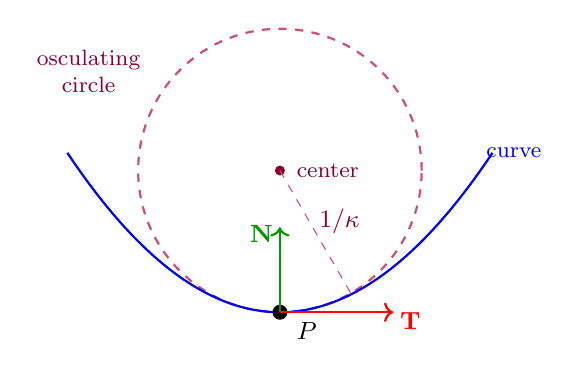
\begin{tikzpicture}[scale=1.8]
    % Osculating circle (dashed)
    \draw[dashed, thick, purple!70] (0, 1) circle (1);
    
    % Circle center
    \fill[purple!70!black] (0, 1) circle (1pt);
    \node[purple!70!black, right, font=\footnotesize] at (0.05, 1) {center};
    
    % Radius line and label
    \draw[dashed, purple!70] (0, 1) -- (0.5, 0.134);
    \node[purple!70!black, font=\small] at (0.42, 0.64) {$1/\kappa$};
    
    % Curve (parabola y = 0.5 x^2)
    \draw[thick, blue, domain=-1.5:1.5, samples=60] plot (\x, {0.5*\x*\x});
    
    % Point P
    \fill (0, 0) circle (1.5pt);
    \node[below right, font=\small] at (0.05, 0) {$P$};
    
    % T arrow (tangent, horizontal)
    \draw[->, red, thick] (0, 0) -- (0.8, 0);
    \node[red, font=\small] at (0.92, -0.06) {$\mathbf{T}$};
    
    % N arrow (normal, upward)
    \draw[->, green!60!black, thick] (0, 0) -- (0, 0.6);
    \node[green!60!black, font=\small] at (-0.13, 0.55) {$\mathbf{N}$};
    
    % Labels
    \node[purple!70!black, font=\footnotesize, align=center] at (-1.35, 1.7) {osculating\\circle};
    \node[blue, font=\footnotesize] at (1.65, 1.125) {curve};
\end{tikzpicture}
\caption{Osculating circle to a curve at point $P$. It is tangent to the curve at $P$, lies in the plane spanned by $\mathbf{T}$ and $\mathbf{N}$, and has radius $1/\kappa$ where $\kappa$ is the curvature of the curve at $P$.}
\label{fig:osculating-circle}
\end{figure}

Lastly, the binormal completes the orthonormal frame as one would expect using the right-hand rule:
$$\mathbf{B}(s) = \mathbf{T}(s) \times \mathbf{N}(s).$$
Together $(\mathbf{T}, \mathbf{N}, \mathbf{B})$ is the \textit{Frenet frame}: an orthonormal basis attached to each point of the curve, oriented to the curve's geometry rather than to the ambient $x, y, z$ axes.

The Frenet-Serret formulas describe how this frame rotates as you slide along the curve:
\begin{align*}
\mathbf{T}'(s) &= \phantom{-}\kappa(s)\, \mathbf{N}(s), \\
\mathbf{N}'(s) &= -\kappa(s)\, \mathbf{T}(s) + \tau(s)\, \mathbf{B}(s), \\
\mathbf{B}'(s) &= -\tau(s)\, \mathbf{N}(s).
\end{align*}
The first follows directly from the definitions of $\mathbf{N}$ and $\kappa$. The new quantity $\tau(s)$ is the \textit{torsion}: it measures how much the curve twists out of its osculating plane. A planar curve has $\tau = 0$ throughout; a generic space curve has nonzero torsion. The third formula can be derived from the first two by differentiating $\mathbf{B} = \mathbf{T} \times \mathbf{N}$ and using the product rule for the cross product.

Let us again revisit the helix. With the unit-speed parametrization 

$\tilde{\gamma}(s) = (\cos(s/\sqrt{2}), \sin(s/\sqrt{2}), s/\sqrt{2})$:
$$\mathbf{T}(s) = \left(-\tfrac{1}{\sqrt{2}}\sin(s/\sqrt{2}),\; \tfrac{1}{\sqrt{2}}\cos(s/\sqrt{2}),\; \tfrac{1}{\sqrt{2}}\right),$$
$$\mathbf{T}'(s) = \left(-\tfrac{1}{2}\cos(s/\sqrt{2}),\; -\tfrac{1}{2}\sin(s/\sqrt{2}),\; 0\right),$$
$$\kappa(s) = |\mathbf{T}'(s)| = \tfrac{1}{2}.$$
The curvature is constant, $\kappa = 1/2$. Normalizing,
$$\mathbf{N}(s) = \left(-\cos(s/\sqrt{2}),\; -\sin(s/\sqrt{2}),\; 0\right),$$
which is a horizontal unit vector pointing inward toward the $z$-axis at every $s$. A short cross-product computation gives the binormal and a constant torsion $\tau = 1/2$. So the helix has constant curvature and constant torsion, which matches its uniform geometric shape.

\begin{figure}[H]
\centering
\begin{tikzpicture}[scale=1.0]
    % A wavy curve
    \draw[thick, blue, domain=-2:3.5, samples=80] plot (\x, {0.6*sin(1.2*\x r) + 0.3*\x});
    % Mark a point
    \def\tval{1.2}
    \pgfmathsetmacro\yval{0.6*sin(1.2*\tval r) + 0.3*\tval}
    \pgfmathsetmacro\dyval{0.72*cos(1.2*\tval r) + 0.3}
    \pgfmathsetmacro\normd{sqrt(1 + \dyval*\dyval)}
    \pgfmathsetmacro\tx{1/\normd}
    \pgfmathsetmacro\ty{\dyval/\normd}
    \fill (\tval, \yval) circle (1.5pt);
    % Tangent arrow
    \draw[->, red, thick] (\tval, \yval) -- ({\tval + 1.3*\tx}, {\yval + 1.3*\ty}) node[above right] {$\mathbf{T}(t)$};
    % Normal arrow (perpendicular)
    \draw[->, green!60!black, thick] (\tval, \yval) -- ({\tval - 1.0*\ty}, {\yval + 1.0*\tx}) node[above left] {$\mathbf{N}(t)$};
\end{tikzpicture}
\caption{A planar curve with its unit tangent $\mathbf{T}$ and unit normal $\mathbf{N}$ at a single point.}
\label{fig:frenet}
\end{figure}

\section{Parametrized Surfaces}

Brownian motion in the project takes place on a parametrized surface in $\mathbb{R}^3$, so understanding what such a surface is, what is considered a regular point, and how to compute the tangent plane and unit normal is the quintessential connection from calculus to the geometry we employ later.

\subsection{Definition and Regular Points}

A \textit{parametrized surface} in $\mathbb{R}^3$ is a smooth map $\boldsymbol{\phi}: U \to \mathbb{R}^3$, where $U \subseteq \mathbb{R}^2$ is an open set. Writing $\boldsymbol{\phi}(u, v) = (\phi^1(u, v), \phi^2(u, v), \phi^3(u, v))$, the partial derivatives
$$\boldsymbol{\phi}_u = \frac{\partial \boldsymbol{\phi}}{\partial u}, \quad \boldsymbol{\phi}_v = \frac{\partial \boldsymbol{\phi}}{\partial v}$$
are vectors in $\mathbb{R}^3$ for each $(u, v) \in U$. They are the two columns of the Jacobian matrix.

A point $(u_0, v_0) \in U$ is called \textit{regular} if $\boldsymbol{\phi}_u(u_0, v_0)$ and $\boldsymbol{\phi}_v(u_0, v_0)$ are linearly independent, or equivalently, if $\boldsymbol{\phi}_u(u_0, v_0) \times \boldsymbol{\phi}_v(u_0, v_0) \neq \mathbf{0}.$
A parametrized surface is \textit{regular} if every point in $U$ is regular. Regularity is the condition that the surface is two-dimensional at the point in question; the two partial-derivative vectors span a plane rather than collapsing onto a line or a point. 

At an irregular point, the parametrization might still describe a geometric surface, but the parametrization itself fails; the standard example is the apex of a cone parametrized in the obvious way.

\subsection{The Tangent Plane and the Unit Normal}

At a regular point $p = \boldsymbol{\phi}(u_0, v_0)$, the \textit{tangent plane} to the surface, denoted $T_p S$, is the two-dimensional subspace of $\mathbb{R}^3$ spanned by $\boldsymbol{\phi}_u$ and $\boldsymbol{\phi}_v$. Every tangent vector at $p$ is a linear combination $a \boldsymbol{\phi}_u + b \boldsymbol{\phi}_v$ for some $a, b \in \mathbb{R}$. This is the multivariable equivalent of the tangent line to a curve from single-variable calculus.

The \textit{unit normal} to the surface at $p$ is the unit vector orthogonal to the tangent plane:
$$\mathbf{N}(p) = \frac{\boldsymbol{\phi}_u \times \boldsymbol{\phi}_v}{|\boldsymbol{\phi}_u \times \boldsymbol{\phi}_v|}.$$
The choice of sign depends on the order of $\boldsymbol{\phi}_u$ and $\boldsymbol{\phi}_v$; swapping them flips $\mathbf{N}$. Once a sign is chosen, $\mathbf{N}(p)$ defines an outward or inward direction at every regular point. Pairing the tangent plane and the unit normal allows us to decompose any vector $\mathbf{v} \in \mathbb{R}^3$ into a tangential part (which lies in $T_p S$) and a normal part (which is parallel to $\mathbf{N}(p)$):
$$\mathbf{v} = \underbrace{\big( \mathbf{v} - (\mathbf{v} \cdot \mathbf{N}) \mathbf{N} \big)}_{\text{tangential}} + \underbrace{(\mathbf{v} \cdot \mathbf{N}) \mathbf{N}}_{\text{normal}}.$$
The tangential part is the orthogonal projection of $\mathbf{v}$ onto $T_p S$, computed via the formula we derived in the linear algebra document. This decomposition is the backbone of the simulator's projection method. At each step, we generate a random vector in $\mathbb{R}^3$, disregard its normal component, and take the tangential part as the random step on the surface.

\begin{figure}[H]
\centering
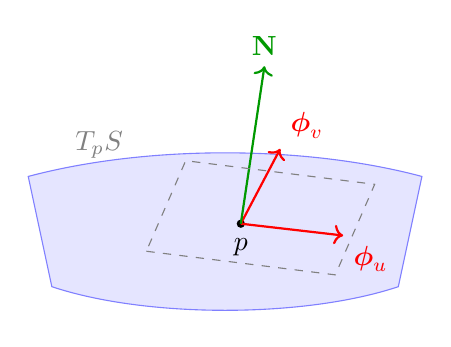
\begin{tikzpicture}[scale=1.0]
    % Surface (curved shape, drawn as a parallelogram with a slight wave)
    \filldraw[fill=blue!10, draw=blue!50] 
        (-2.2, -0.8) .. controls (-1, -1.2) and (1, -1.2) .. (2.2, -0.8)
        -- (2.5, 0.6) .. controls (1, 1.0) and (-1, 1.0) .. (-2.5, 0.6) -- cycle;
    % Point p
    \fill (0.2, 0) circle (1.5pt) node[below=2pt] {$p$};
    % Tangent vectors phi_u and phi_v
    \draw[->, red, thick] (0.2, 0) -- (1.5, -0.15) node[below right] {$\boldsymbol{\phi}_u$};
    \draw[->, red, thick] (0.2, 0) -- (0.7, 0.95) node[above right] {$\boldsymbol{\phi}_v$};
    % Normal vector
    \draw[->, green!60!black, thick] (0.2, 0) -- (0.5, 2.0) node[above] {$\mathbf{N}$};
    % Tangent plane (light gray quadrilateral)
    \draw[dashed, gray] (-1.0, -0.35) -- (1.4, -0.65) -- (1.9, 0.5) -- (-0.5, 0.8) -- cycle;
    \node[gray] at (-1.6, 1.0) {$T_p S$};
\end{tikzpicture}
\caption{A parametrized surface near a regular point $p$. The tangent vectors $\boldsymbol{\phi}_u, \boldsymbol{\phi}_v$ span the tangent plane $T_p S$; the unit normal $\mathbf{N}$ is perpendicular to it.}
\label{fig:tangent-plane}
\end{figure}

\subsection{Two Worked Examples: $S^2$ and $T^2$}

\textbf{The Sphere.} The standard parametrization of the unit sphere $S^2 \subset \mathbb{R}^3$ in spherical coordinates is
$$\boldsymbol{\phi}(\theta, \varphi) = (\sin\theta \cos\varphi,\; \sin\theta \sin\varphi,\; \cos\theta), \quad (\theta, \varphi) \in (0, \pi) \times [0, 2\pi).$$
Here $\theta$ is the polar angle (measured from the north pole) and $\varphi$ is the azimuthal angle. Computing the partial derivatives,
\begin{align*}
\boldsymbol{\phi}_\theta &= (\cos\theta \cos\varphi,\; \cos\theta \sin\varphi,\; -\sin\theta), \\
\boldsymbol{\phi}_\varphi &= (-\sin\theta \sin\varphi,\; \sin\theta \cos\varphi,\; 0).
\end{align*}
A short computation gives the cross product $\boldsymbol{\phi}_\theta \times \boldsymbol{\phi}_\varphi = \sin\theta \cdot \boldsymbol{\phi}$ and the magnitude $|\boldsymbol{\phi}_\theta \times \boldsymbol{\phi}_\varphi| = \sin\theta$. Hence the unit normal at a point $\boldsymbol{\phi}(\theta, \varphi)$ is
$$\mathbf{N} = \boldsymbol{\phi}(\theta, \varphi),$$
which is to say, the unit normal at any point on the unit sphere is the position vector of that point. Substituting this into the orthogonal-projection formula from the previous subsection gives
$$\mathbf{v}_{\text{tangential}} = \mathbf{v} - (\mathbf{v} \cdot \mathbf{x}) \mathbf{x}, \quad \mathbf{x} \in S^2,$$
which is the formula the simulator uses to project a random Gaussian vector onto the tangent plane at the current point. The parametrization fails (is irregular) at the poles, where $\sin\theta = 0$ and $\boldsymbol{\phi}_\varphi = \mathbf{0}$; this is a standard coordinate-chart artifact, not a real geometric problem.

textbf{The Torus.} The standard parametrization of the torus of major radius $R$ (distance from the center of the tube to the central $z$-axis) and minor radius $r$ (radius of the tube itself) is
$$\boldsymbol{\phi}(u, v) = \big((R + r\cos v)\cos u,\; (R + r\cos v)\sin u,\; r\sin v\big), \quad (u, v) \in [0, 2\pi) \times [0, 2\pi).$$
Here $u$ is the angle around the central $z$-axis (going around the big loop) and $v$ is the angle around the tube's cross-section (going around the small loop). Computing the partial derivatives,
\begin{align*}
\boldsymbol{\phi}_u &= \big(-(R + r\cos v)\sin u,\; (R + r\cos v)\cos u,\; 0\big), \\
\boldsymbol{\phi}_v &= \big(-r\sin v\cos u,\; -r\sin v\sin u,\; r\cos v\big).
\end{align*}
The cross product factors cleanly:
$$\boldsymbol{\phi}_u \times \boldsymbol{\phi}_v = r(R + r\cos v)\big(\cos v\cos u,\; \cos v\sin u,\; \sin v\big).$$
The vector in parentheses has unit length (verify: $\cos^2 v\cos^2 u + \cos^2 v\sin^2 u + \sin^2 v = \cos^2 v + \sin^2 v = 1$), so
$$|\boldsymbol{\phi}_u \times \boldsymbol{\phi}_v| = r(R + r\cos v),$$
and the unit normal is
$$\mathbf{N}(u, v) = \big(\cos v\cos u,\; \cos v\sin u,\; \sin v\big).$$
Two observations are worth recording. First, the cross product magnitude is not constant: it is largest on the outer equator ($v = 0$, where it equals $r(R + r)$) and smallest on the inner equator ($v = \pi$, where it equals $r(R - r)$). This non-uniformity is the reason the invariant measure of Brownian motion on the embedded torus is not uniform in $(u, v)$ coordinates, a fact the project flags repeatedly. Second, the parametrization is regular at every $(u, v)$, assuming $R > r$ so that $R + r\cos v > 0$ everywhere. This is a cleaner situation than the sphere, where the poles required a separate chart.
 
\begin{figure}[H]
\centering
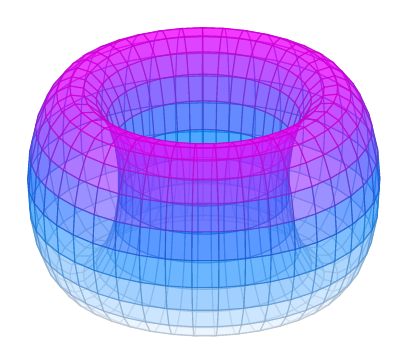
\begin{tikzpicture}
\begin{axis}[
    view={50}{40},
    width=0.65\textwidth,
    axis lines=none,
    ticks=none,
    z buffer=sort,
    enlargelimits=false,
    domain=0:360, y domain=0:360,
    samples=42, samples y=22,
]
\addplot3[surf, opacity=0.65, fill opacity=0.55,
          colormap/cool, shader=faceted]
    ({(2 + 0.7*cos(y))*cos(x)}, {(2 + 0.7*cos(y))*sin(x)}, {0.7*sin(y)});
\end{axis}
\end{tikzpicture}
\caption{The torus of major radius $R$ and minor radius $r$ (drawn with $R = 2, r = 0.7$). The parameter $u$ runs around the central $z$-axis (the big loop); $v$ runs around the tube cross-section (the small loop).}
\label{fig:torus-3d}
\end{figure}
 
\section{Multiple Integrals and the Change of Variables Formula}
 
\subsection{Iterated Integrals and Fubini's Theorem}
 
The double integral $\iint_R f(x, y)\, dA$ of a continuous function over a region $R \subseteq \mathbb{R}^2$ can be computed as an iterated integral $\int \!\!\int f(x, y)\, dy\, dx$, with the order of integration swappable under the conditions of Fubini's theorem. The same idea extends to triple and higher integrals.
 
\subsection{The Change of Variables Formula}
 
If $\mathbf{T}: U \to V$ is a smooth invertible map between open subsets of $\mathbb{R}^n$ with Jacobian determinant $\det D\mathbf{T}(\mathbf{u})$ nonzero everywhere, then for any integrable $f: V \to \mathbb{R}$,
$$\int_V f(\mathbf{x})\, d\mathbf{x} = \int_U f(\mathbf{T}(\mathbf{u})) \cdot |\det D\mathbf{T}(\mathbf{u})|\, d\mathbf{u}.$$
The Jacobian determinant is the local volume-distortion factor of $\mathbf{T}$. It measures how much $\mathbf{T}$ stretches or shrinks small volumes near $\mathbf{u}$.
 
\textit{Worked example: polar coordinates.} The map $\mathbf{T}(r, \theta) = (r\cos\theta,\, r\sin\theta)$ has Jacobian matrix
$$D\mathbf{T} = \begin{pmatrix} \cos\theta & -r\sin\theta \\ \sin\theta & \phantom{-}r\cos\theta \end{pmatrix}, \qquad \det D\mathbf{T} = r\cos^2\theta + r\sin^2\theta = r.$$
Hence the change-of-variables formula gives $dA = r\, dr\, d\theta$, the familiar polar area element. The factor of $r$ is a result of the Jacobian determinant accounting for the fact that a thin polar wedge of width $d\theta$ and radial extent $dr$ has Euclidean area $r\, dr\, d\theta$, not $dr\, d\theta$, since the arc length swept out at radius $r$ is $r\, d\theta$.
 
A famous application is the Gaussian integral $I = \int_{-\infty}^\infty e^{-x^2}\, dx$. Squaring,
$$I^2 = \int_{-\infty}^\infty\!\!\int_{-\infty}^\infty e^{-(x^2 + y^2)}\, dx\, dy.$$
This double integral is intractable in Cartesian coordinates, but in polar it becomes
$$I^2 = \int_0^{2\pi}\!\!\int_0^\infty e^{-r^2}\, r\, dr\, d\theta = 2\pi \cdot \tfrac{1}{2} = \pi,$$
so $I = \sqrt{\pi}$. The change-of-variables formula turns a hard integral into a one-line computation, and the entire trick is the appearance of the factor $r$.

\textbf{The Significance of the Volume-Distortion Factor.} The change-of-variables formula is what makes the volume form $\sqrt{|g|}\, du\, dv$ an accurate measure on a surface. If we omit the Jacobian determinant when  changing coordinates, probability densities will not normalize and our simulator will report the wrong invariant measure on $T^2$. With this in mind, we shall circumvent this pitfall when we encounter the torus.
 
\section{The Surface Area Element and Surface Integrals}
  
\subsection{The Surface Area Element}
 
For a parametrized surface $\boldsymbol{\phi}: U \to \mathbb{R}^3$, the area element is
$$dA = |\boldsymbol{\phi}_u \times \boldsymbol{\phi}_v|\, du\, dv,$$
and the total surface area is $\iint_U |\boldsymbol{\phi}_u \times \boldsymbol{\phi}_v|\, du\, dv$.
 
For the sphere $S^2$, the cross-product magnitude from Section 5.3 is $\sin\theta$, so
$$\text{Area}(S^2) = \int_0^{2\pi}\!\!\int_0^\pi \sin\theta\, d\theta\, d\varphi = 2\pi \cdot 2 = 4\pi,$$
which recovers the standard surface area of the unit sphere.
 
For the torus with major radius $R$ and minor radius $r$, the cross-product magnitude is $r(R + r\cos v)$, so
$$\text{Area}(T^2) = \int_0^{2\pi}\!\!\int_0^{2\pi} r(R + r\cos v)\, du\, dv = 2\pi r \int_0^{2\pi}(R + r\cos v)\, dv = 2\pi r \cdot 2\pi R = 4\pi^2 R r,$$
since $\int_0^{2\pi}\cos v\, dv = 0$. The surface-area of $4\pi^2$ is an interesting property affirming the torus is topologically a product of two circles.
 
\subsection{Surface Integrals of Scalar Functions}
 
The surface integral of a scalar function $f: \mathbb{R}^3 \to \mathbb{R}$ over a parametrized surface $S$ is
$$\iint_S f\, dA = \iint_U f(\boldsymbol{\phi}(u, v)) \cdot |\boldsymbol{\phi}_u \times \boldsymbol{\phi}_v|\, du\, dv.$$
As an example, compute the average value of $z$ over $S^2$. On the sphere, $z = \cos\theta$, so
$$\bar{z} = \frac{1}{4\pi}\int_{S^2} z\, dA = \frac{1}{4\pi}\int_0^{2\pi}\!\!\int_0^\pi \cos\theta \cdot \sin\theta\, d\theta\, d\varphi = \frac{2\pi}{4\pi}\int_0^\pi \tfrac{1}{2}\sin(2\theta)\, d\theta = 0,$$
since $\sin(2\theta)$ integrated over a half-period of $2\theta$ vanishes. By symmetry, $\bar{x} = \bar{y} = 0$ as well, so the centroid of the unit sphere's surface is the origin, consistent with the sphere's rotational symmetry.
 
\section{Vector Calculus Operators}
  
\subsection{Divergence}
 
For a vector field $\mathbf{F}: \mathbb{R}^n \to \mathbb{R}^n$ with components $\mathbf{F} = (F_1, \ldots, F_n)$, the \textit{divergence} is the scalar function
$$\nabla \cdot \mathbf{F} = \sum_{i=1}^n \frac{\partial F_i}{\partial x_i}.$$
 
A physical equivalent is fluid flow. Think of $\mathbf{F}(\mathbf{x})$ as the velocity of a fluid (say, water or gas) at the point $\mathbf{x}$. Then $\nabla \cdot \mathbf{F}(\mathbf{a})$ measures the net rate at which fluid is flowing out of a tiny region around $\mathbf{a}$, per unit volume of that region. Three cases:
 
If $\nabla \cdot \mathbf{F}(\mathbf{a}) > 0$, more fluid leaves a tiny region than enters it. The point acts as a \textit{source}, like a faucet pumping fluid into the space.
 
If $\nabla \cdot \mathbf{F}(\mathbf{a}) < 0$, more fluid enters a tiny region than leaves. The point acts as a \textit{sink}, like a drain.
 
If $\nabla \cdot \mathbf{F}(\mathbf{a}) = 0$, inflow exactly matches outflow. The fluid is incompressible at that point, with no source or sink there.
 
Some examples in $\mathbb{R}^2$:
 
\textbf{Radial outward.} For $\mathbf{F}(x, y) = (x, y)$, the arrows point straight away from the origin and grow longer with distance. Computing,
$$\nabla \cdot \mathbf{F} = \frac{\partial x}{\partial x} + \frac{\partial y}{\partial y} = 1 + 1 = 2.$$
The divergence is constant and positive: every point is a source. Imagine water gushing out of every point of the plane simultaneously.
 
\textbf{Constant flow.} For $\mathbf{F}(x, y) = (1, 0)$, all arrows are unit-length pointing right. The divergence is $0 + 0 = 0$. No sources or sinks anywhere; fluid simply flows through each region at constant rate, with as much entering on the left as exiting on the right.
 
\textbf{Hyperbolic flow.} For $\mathbf{F}(x, y) = (x, -y)$, fluid stretches outward along the $x$-axis and is compressed inward along the $y$-axis. Divergence: $1 + (-1) = 0$. Net inflow in $y$ exactly cancels net outflow in $x$, so there is no local source or sink, even though the field is doing something visibly nontrivial.
 
\textbf{Rotational flow. }For $\mathbf{F}(x, y) = (-y, x)$, arrows swirl counterclockwise around the origin. Divergence: $0 + 0 = 0$. Pure rotation has zero divergence: it shuffles fluid around without compressing or expanding it anywhere.
 
\subsection{Curl}
 
The \textit{curl} of a vector field, defined in $\mathbb{R}^3$, is the vector field
$$\nabla \times \mathbf{F} = \left(\frac{\partial F_3}{\partial y} - \frac{\partial F_2}{\partial z},\; \frac{\partial F_1}{\partial z} - \frac{\partial F_3}{\partial x},\; \frac{\partial F_2}{\partial x} - \frac{\partial F_1}{\partial y}\right).$$
The curl is itself a vector field, not a scalar.
 
Another physical equivalent: imagine placing a tiny paddlewheel at a point $\mathbf{a}$, free to spin about any axis through $\mathbf{a}$. The curl vector $\nabla \times \mathbf{F}(\mathbf{a})$ points along the axis about which the paddlewheel spins fastest, with orientation given by the right-hand rule (fingers curl with the direction of rotation; thumb points along the curl). The magnitude $|\nabla \times \mathbf{F}(\mathbf{a})|$ is twice the angular velocity of the wheel.
 
\textbf{Rotation around the $z$-axis}. For $\mathbf{F}(x, y, z) = (-y, x, 0)$, arrows swirl counterclockwise in horizontal planes. Computing,
$$\nabla \times \mathbf{F} = (0 - 0,\; 0 - 0,\; 1 - (-1)) = (0, 0, 2).$$
The curl points in $+\hat{\mathbf{z}}$ with magnitude $2$: the paddlewheel at any point spins counterclockwise (viewed from above) about the vertical axis. This matches the visible bulk rotation of the fluid.
 
\textbf{Radial outward.} For $\mathbf{F}(x, y, z) = (x, y, z)$, the field is purely radial. Each component of the curl involves derivatives of one coordinate with respect to another (e.g., $\partial F_3 / \partial y = \partial z / \partial y = 0$), all of which vanish. Hence $\nabla \times \mathbf{F} = \mathbf{0}$. In this case, the paddlewheel does not spin. The fluid expands outward but does not rotate.
 
\textbf{\textit{Shear flow.} }For $\mathbf{F}(x, y, z) = (y, 0, 0)$, the field points in the $+x$ direction with magnitude $|y|$; above the $x$-axis fluid moves right, below it moves left. Computing,
$$\nabla \times \mathbf{F} = (0 - 0,\; 0 - 0,\; 0 - 1) = (0, 0, -1).$$
The curl points in $-\hat{\mathbf{z}}$. A paddlewheel with vertical axis placed at any point spins clockwise (viewed from above), because the top blade is pushed right faster than the bottom blade. This is a key example of a field with no visible, large-scale swirl but nonzero curl. The rotation is local, arising from the velocity gradient across the wheel rather than any ''pure'' circulation.
 
\begin{figure}[H]
\centering
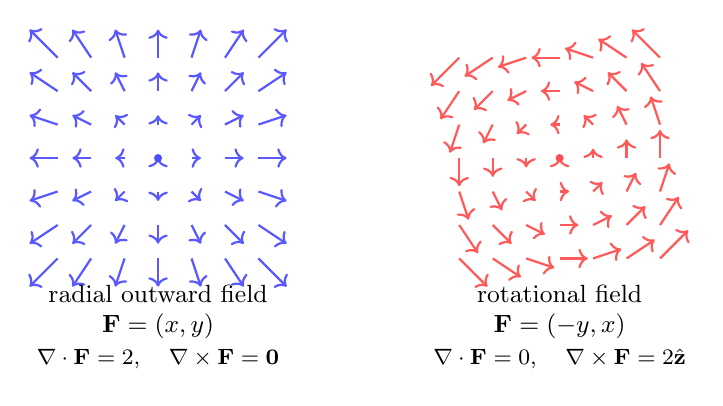
\begin{tikzpicture}[scale=0.85]
% LEFT: F = (x, y), radial outward, centered at (-3, 0)
\foreach \i in {-1.5, -1, -0.5, 0, 0.5, 1, 1.5}{
  \foreach \j in {-1.5, -1, -0.5, 0, 0.5, 1, 1.5}{
    \pgfmathsetmacro\fx{0.28*\i}
    \pgfmathsetmacro\fy{0.28*\j}
    \draw[->, blue!65, thick] ({-3 + \i}, \j) -- ({-3 + \i + \fx}, {\j + \fy});
  }
}
\fill[blue!70] (-3, 0) circle (1.7pt);
\node[align=center, font=\small] at (-3, -2.3) {radial outward field\\$\mathbf{F} = (x, y)$};
\node[align=center, font=\footnotesize] at (-3, -3.0) {$\nabla\cdot\mathbf{F} = 2$, \;\; $\nabla\times\mathbf{F} = \mathbf{0}$};
 
% RIGHT: F = (-y, x), rotational, centered at (3, 0)
\foreach \i in {-1.5, -1, -0.5, 0, 0.5, 1, 1.5}{
  \foreach \j in {-1.5, -1, -0.5, 0, 0.5, 1, 1.5}{
    \pgfmathsetmacro\fx{-0.28*\j}
    \pgfmathsetmacro\fy{0.28*\i}
    \draw[->, red!65, thick] ({3 + \i}, \j) -- ({3 + \i + \fx}, {\j + \fy});
  }
}
\fill[red!70] (3, 0) circle (1.7pt);
\node[align=center, font=\small] at (3, -2.3) {rotational field\\$\mathbf{F} = (-y, x)$};
\node[align=center, font=\footnotesize] at (3, -3.0) {$\nabla\cdot\mathbf{F} = 0$, \;\; $\nabla\times\mathbf{F} = 2\hat{\mathbf{z}}$};
\end{tikzpicture}
\caption{Two contrasting vector fields, each arrow anchored at the lattice point with length and direction showing the field at that point. The radial field (left) has positive divergence everywhere (every point is a source) and zero curl (a paddlewheel placed in this flow would not spin). The rotational field (right) has zero divergence (no expansion or compression anywhere) and constant nonzero curl (a paddlewheel spins about the vertical axis).}
\label{fig:div-curl}
\end{figure}
 
\subsection{The Laplacian in $\mathbb{R}^n$}
 
The \textit{Laplacian} of a scalar function $f: \mathbb{R}^n \to \mathbb{R}$ is
$$\Delta f = \nabla \cdot \nabla f = \sum_{i=1}^n \frac{\partial^2 f}{\partial x_i^2}.$$
It is the divergence of the gradient. In one variable, $\Delta f = f''$, so the Laplacian generalizes the second derivative from single-variable calculus.
 
A straightforward geometric interpretation of the Laplacian is that it measures how much $f$ at a point differs from the average value of $f$ in a small neighborhood of that point. Precisely, in $\mathbb{R}^2$, averaging $f$ over a small disk of radius $\rho$ around $\mathbf{a}$ has the expansion
$$\underbrace{\frac{1}{\pi\rho^2}\int_{B(\mathbf{a}, \rho)} f\, dA}_{\text{average of } f \text{ near } \mathbf{a}} = f(\mathbf{a}) + \frac{\rho^2}{8}\Delta f(\mathbf{a}) + O(\rho^4).$$
(The constant depends on the dimension.) Reading off the sign of $\Delta f(\mathbf{a})$:
 
If $\Delta f(\mathbf{a}) > 0$, the local average of $f$ near $\mathbf{a}$ exceeds $f(\mathbf{a})$. The value at the point is below the local average. Any local minimum satisfies $\Delta f > 0$.
 
If $\Delta f(\mathbf{a}) < 0$, the value at the point exceeds the local average. Any local maximum satisfies $\Delta f < 0$.
 
If $\Delta f(\mathbf{a}) = 0$, the function value at the point matches the local average. Functions for which $\Delta f \equiv 0$ everywhere are called \textit{harmonic}, and they satisfy the \textit{mean-value property}: $f(\mathbf{a})$ equals the average of $f$ over any small symmetric region centered at $\mathbf{a}$.
 
Examples.

\textit{(1)} $f(x, y) = x^2 + y^2$ has $\Delta f = 2 + 2 = 4 > 0$. The function has a minimum at the origin; nearby values are all higher than $f(0,0) = 0$. The Laplacian is positive.
 
\textit{(2)} $f(x, y) = -(x^2 + y^2)$ has $\Delta f = -4 < 0$. Maximum at the origin; nearby values are lower; the Laplacian is negative.
 
\textit{(3)} $f(x, y) = x^2 - y^2$ has $\Delta f = 2 - 2 = 0$. The function is harmonic, even though it has a saddle at the origin. The concavity in $x$ exactly cancels the concavity in $y$, so the function's average over any small disk centered at the origin equals $f(0,0) = 0$.
 
\textit{(4)} Any affine function $f(\mathbf{x}) = \mathbf{a}\cdot\mathbf{x} + b$ has $\Delta f = 0$. The average of an affine function over a symmetric region is its value at the center.
 
\textit{Why this is the right operator for diffusion.} The heat equation in $\mathbb{R}^n$ is
$$\frac{\partial u}{\partial t}(\mathbf{x}, t) = \tfrac{1}{2}\,\Delta u(\mathbf{x}, t),$$
where $u(\mathbf{x}, t)$ is, say, the temperature at position $\mathbf{x}$ and time $t$. The reason this is the correct equation follows directly from the mean-value intuition. Heat flows from hot regions to cold regions, so the rate of temperature change at a point depends on how the point compares to its surroundings:
 
If $u(\mathbf{a})$ is below the local average ($\Delta u > 0$), heat flows in and the temperature there rises, giving $\partial u / \partial t > 0$.
 
If $u(\mathbf{a})$ is above the local average ($\Delta u < 0$), heat flows out and the temperature falls, giving $\partial u / \partial t < 0$.
 
If $u(\mathbf{a})$ equals the local average ($\Delta u = 0$), nothing changes at that instant.
 
So temperature evolves toward the local average at a rate proportional to $\Delta u$.
 
\textit{Connection to Brownian motion.} The probability density of a Brownian particle's position at time $t$ satisfies the same heat equation because a Brownian particle takes a random step of equal likelihood in every direction at each instant, so the density at a point increases when neighboring densities are higher than the point's own and decreases when they are lower. The Laplacian is thus ``how a function compares to its local average,'' which is why $\tfrac{1}{2}\Delta$ is the infinitesimal generator of Brownian motion in $\mathbb{R}^n$.
 
On a curved surface, the analog of $\Delta$ is the \textit{Laplace-Beltrami operator}, $\Delta_g$. It is built from the metric tensor $g_{ij}$ via the same divergence-of-gradient construction, but with the divergence and gradient taken intrinsically (using a metric of the surface rather than the Euclidean dot product). The generator of Brownian motion on a Riemannian manifold is $\tfrac{1}{2}\Delta_g$,  and we shall study this further.

\end{document}
